\documentclass{../TexTemplate/myslide}
\usepackage[slide,table,cpp]{../TexTemplate/mypackage}
\hypersetup{colorlinks=true,linkcolor=black,urlcolor=blue}
\usepackage{xcolor}

\renewcommand{\thefootnote}{\fnsymbol{footnote}}

\title[ToolsSeminar]{Tools Seminar}
\subtitle{Week 10 - Parallel Computing}
\author[chhzh123]{Hongzheng~Chen}
\date[Mar 30, 2020]{Mar 30, 2020}

\begin{document}

\begin{frame}
\titlepage
\end{frame}

\begin{frame}
\tableofcontents
\end{frame}

\section{Introduction}
\begin{frame}
\sectionpage
\end{frame}

\begin{frame}
\begin{figure}
\centering
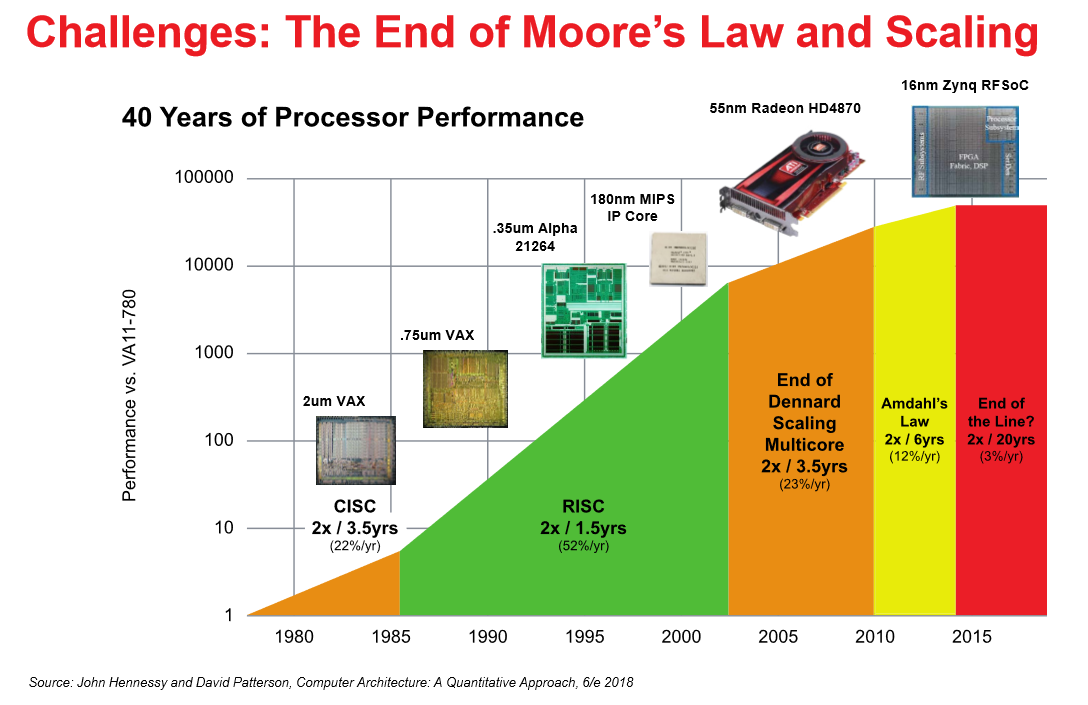
\includegraphics[width=\linewidth]{fig/the_end_of_moores_law_and_scaling.png}
\end{figure}
* That's why \href{https://en.wikipedia.org/wiki/Tick\%E2\%80\%93tock_model}{Intel} is called ``toothpaste factory'' now
% http://blog.peddy.ai/2019/04/03/evolution-of-hardware-for-deep-learning/
\end{frame}

\begin{frame}{The End of Moore's Law and Scaling}
\begin{quote}
This shift toward \textbf{increasing parallelism} is not a triumphant stride forward based on breakthroughs in novel software and architectures for parallelism;
instead, this plunge into parallelism is actually a \textbf{retreat} from even greater challenges that thwart efficient silicon implementation of traditional uniprocessor architectures.\\
\hfill ---  \emph{The Landscape of Parallel Computing Research: A View from Berkeley}, 2006
\end{quote}
\pause
Thus, multicore processors put burdens from hardware to software, which needs programmers to code parallel programs.
\end{frame}

\begin{frame}{Different hardware}
\begin{figure}[H]
\centering
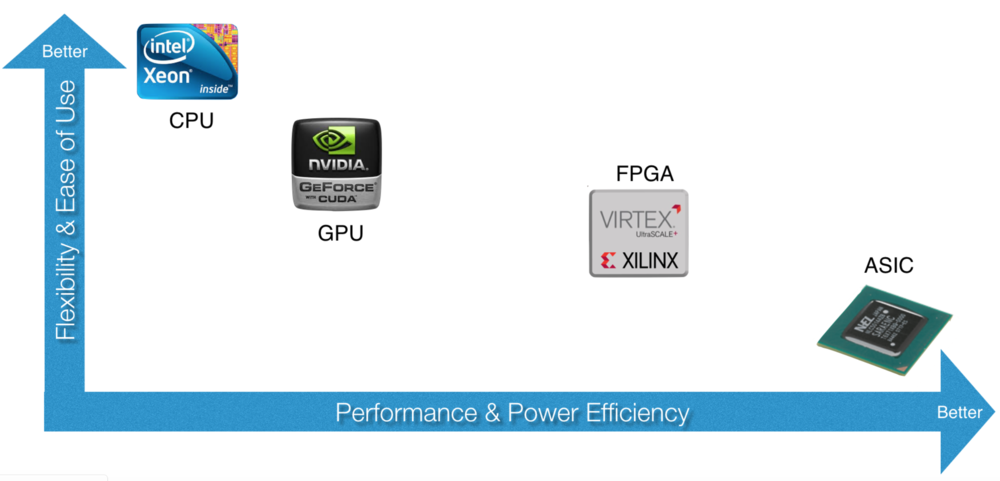
\includegraphics[width=0.8\linewidth]{fig/accelerator_comparison.png}
\end{figure}
\begin{itemize}
	\item CPU
	\item GPU (Graphical Processing Unit)
	\item FPGA (Field-Programmable Gate Array)
	\item ASIC (Application-Specific Integrated Circuit)
\end{itemize}
\end{frame}

\begin{frame}{CPU Architecture}
\begin{figure}
\centering
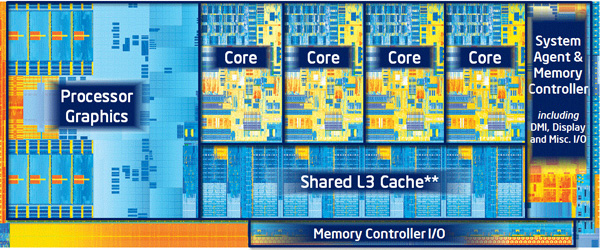
\includegraphics[width=0.9\linewidth]{fig/Intel-core-i7-cpu-die.jpg}
\caption*{\small Intel core i7 CPU (Ivy Bridge)}
% https://www.anandtech.com/Show/Index/5771?cPage=10&all=False&sort=0&page=3&slug=the-intel-ivy-bridge-core-i7-3770k-review
\end{figure}
\end{frame}

\begin{frame}
\begin{figure}
\centering
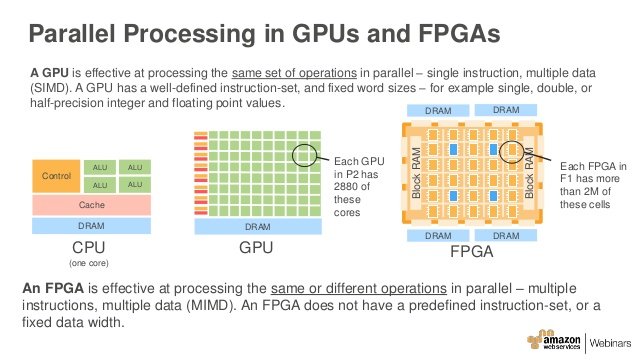
\includegraphics[width=\linewidth]{fig/gpu-fpga.jpg}
\end{figure}
\pause
We will focus on CPU parallelization in this seminar
\end{frame}

\section{Single Machine Parallelization}
\begin{frame}
\sectionpage
\end{frame}

\subsection{Multi-threads}
\begin{frame}
\subsectionpage
\end{frame}

\begin{frame}{Fork-Join Model}
\begin{figure}
\centering
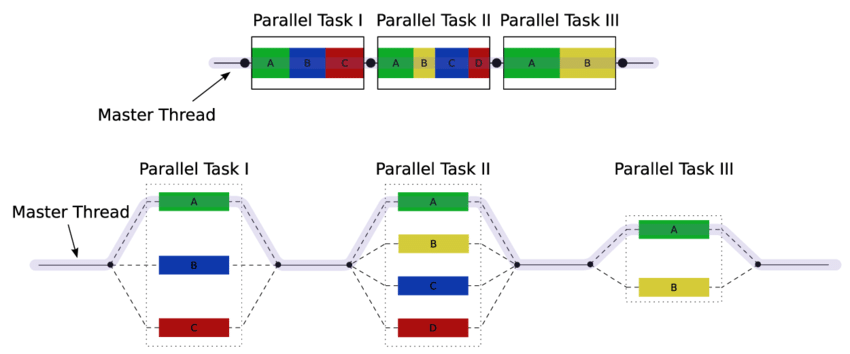
\includegraphics[width=\linewidth]{fig/fork-join.png}
\end{figure}
\begin{itemize}
	\item Fork: Dispatch tasks to each processor / thread
	\item Join: Synchronization, wait till all threads are done
\end{itemize}
\end{frame}

% https://chhzh123.github.io/blogs/2019-03-14-cpp-multithreading/
\begin{frame}[fragile]{pthread}
\href{https://en.wikipedia.org/wiki/POSIX_Threads}{POSIX} (Portable Opearing System Interface for Unix)
\begin{itemize}
\item \verb'<pthread.h>' is in Linux's system library and can be directly called
\end{itemize}
\begin{lstlisting}[basicstyle=\scriptsize]
void *foo(void *arg)
{
	int* id = (int*) arg;
	printf("My id is %d\n", *id);
}

int main()
{
	pthread_t id[4];
	for (int i = 0; i < 4; ++i)
		// pass in function pointer and args
		pthread_create(&id[i],NULL,foo,&i);
	for (int i = 0; i < 4; ++i)
		pthread_join(&id[i],NULL);
	for (int i = 0; i < 4; ++i)
		pthread_exit(&id[i]);
}
\end{lstlisting}
Need to add \verb'-lpthread' flag when compiling
\end{frame}

\begin{frame}[fragile]{<thread>}
C++11 adds initial support for multi-threading in stl
\begin{lstlisting}
#include <iostream>
#include <thread>
using namespace std;

void exec(int n){
	cout << "My id is" << n << endl;
}

int main(){
	thread myThread[4];
	for (int i = 0; i < 4; ++i)
		myThread = thread(exec,i);
	for (int i = 0; i < 4; ++i)
		myThread[i].join();
}
\end{lstlisting}
\end{frame}

\begin{frame}{Race Condition}
Be careful of the shared data
\begin{center}
\begin{tabular}{c|c}
Thread A & Thread B\\
$\cdots$ & $\cdots$\\
Count$++$ & Count$--$\\
$\cdots$ & $\cdots$
\end{tabular}\quad
\begin{tabular}{ll|ll}
Thread A & & Thread B\\
Load & Count & Load & Count\\
Add & \#1 & Sub & \#1\\
Store & Count & Store & Count
\end{tabular}
\end{center}
\begin{itemize}
	\item Critical section: That part of the program where the shared memory is accessed
	\item Need to avoid conflicts and make data consistent
\end{itemize}
\end{frame}

\begin{frame}{Avoid Race Condition}
Two basic methods:
\begin{itemize}
	\item Corse-grained: Lock/mutex
	\item Fine-grained: Atomic operations
\end{itemize}
* There are lots of details about synchronization \& consistency, please refer to books of OS
\end{frame}

\begin{frame}[fragile]{Mutex Operations in pthread}
\verb'<pthread.h>'
\begin{itemize}
\item \verb'pthread_mutex_init(&mutex1,NULL)'
\item \verb'pthread_mutex_destroy(&mutex1)'
\item \verb'pthread_mutex_lock(&mutex1)'
\item \verb'pthread_mutex_unlock(&mutex1)'
\end{itemize}
\verb'<thread>'
\begin{itemize}
	\item \verb'std::mutex g_display_mutex'
	\item \verb'std::lock_guard<std::mutex> guard(g_display_mutex)'
\end{itemize}
\end{frame}

\subsection{OpenMP}
\begin{frame}
\subsectionpage
\end{frame}

% https://chhzh123.github.io/summary/parallel-computing/openmp/
\begin{frame}{OpenMP}
\href{https://www.openmp.org/}{OpenMP} (Open Multi-Processing): Shared-memory programming model
\begin{itemize}
	\item Set of parallel commands, library, and routines
	\item Simplify multi-threading programming
	\item A spec suitable for different devices from desktop to supercomputer
	\item gcc has initial support for OpenMP
\end{itemize}
\end{frame}

\begin{frame}[fragile]{OpenMP API}
\verb'#include <omp.h>' and only need to write compilation directives
\begin{center}
\verb'#pragma omp <directive-name> [clause,...]'
\end{center}
\begin{itemize}
	\item \verb'omp_get_thread_num'
	\item \verb'omp_get/set_num_procs'
	\item \verb'omp_get/set_num_threads'
	\item \verb'#pragma omp parallel for': The most commonly used!
	\item \verb'#pragma omp ... private (<variable list>)'
	\item \verb'#pragma omp ... reduction (op:list)'
\end{itemize}
\end{frame}

\begin{frame}[fragile]{OpenMP Example (Matrix Multiplication)}
\begin{lstlisting}
# pragma omp for
for ( i = 0; i < n; i++ )
{
  for ( j = 0; j < n; j++ )
  {
    c[i][j] = 0.0;
    for ( k = 0; k < n; k++ )
    {
      c[i][j] = c[i][j] + a[i][k] * b[k][j];
    }
  }
}
\end{lstlisting}
\end{frame}

\begin{frame}[fragile]{OpenMP Example (Summation)}
\begin{lstlisting}
float sum(const float *a, size_t n)
{
    float total = 0.;

    #pragma omp parallel for reduction(+:total)
    for (size_t i = 0; i < n; i++) {
        total += a[i];
    }
    return total;
}
\end{lstlisting}
\end{frame}

\subsection{Cilk}
\begin{frame}
\subsectionpage
\end{frame}

% https://chhzh123.github.io/summary/parallel-computing/cilk/
\begin{frame}[fragile]{Intel Clik Plus}
Intel Cilk Plus: A extremely light-weighted parallel framework
\begin{itemize}
	\item \verb'#include<cilk/cilk.h>'
	\item gcc 5.0+: \verb'g++ -O3 -fcilkplus -lcilkrts <source>'
	\item Or compiled by Intel Compiler (icpc) --- Better choice!
	\begin{itemize}
		\item But from icpc 18.0, Intel uses \href{https://software.intel.com/en-us/articles/migrate-your-application-to-use-openmp-or-intelr-tbb-instead-of-intelr-cilktm-plus?_ga=2.174275746.1279103381.1550824040-508775473.1544510410}{Thread Building Block} (TBB)
	\end{itemize}
\end{itemize}
Only three keywords
\begin{itemize}
	\item \verb'cilk_spawn': fork
	\item \verb'cilk_sync': join
	\item \verb'cilk_for': \verb'parallel for'
\end{itemize}
\end{frame}

\begin{frame}[fragile]{Clik Example (Fibbonacci)}
\begin{lstlisting}
int fib(int n)
{
    if (n < 2)
        return n;
    int x = fib(n-1);
    int y = fib(n-2);
    return x + y;
}

int fib(int n)
{
    if (n < 2)
        return n;
    int x = cilk_spawn fib(n-1);
    int y = fib(n-2);
    cilk_sync;
    return x + y;
}
\end{lstlisting}
\end{frame}

\begin{frame}{Cilk Runtime}
The most powerful thing is Cilk runtime deploys \textbf{work-stealing} scheduling strategy, which greatly outperforms OpenMP's runtime
\begin{figure}[H]
\centering
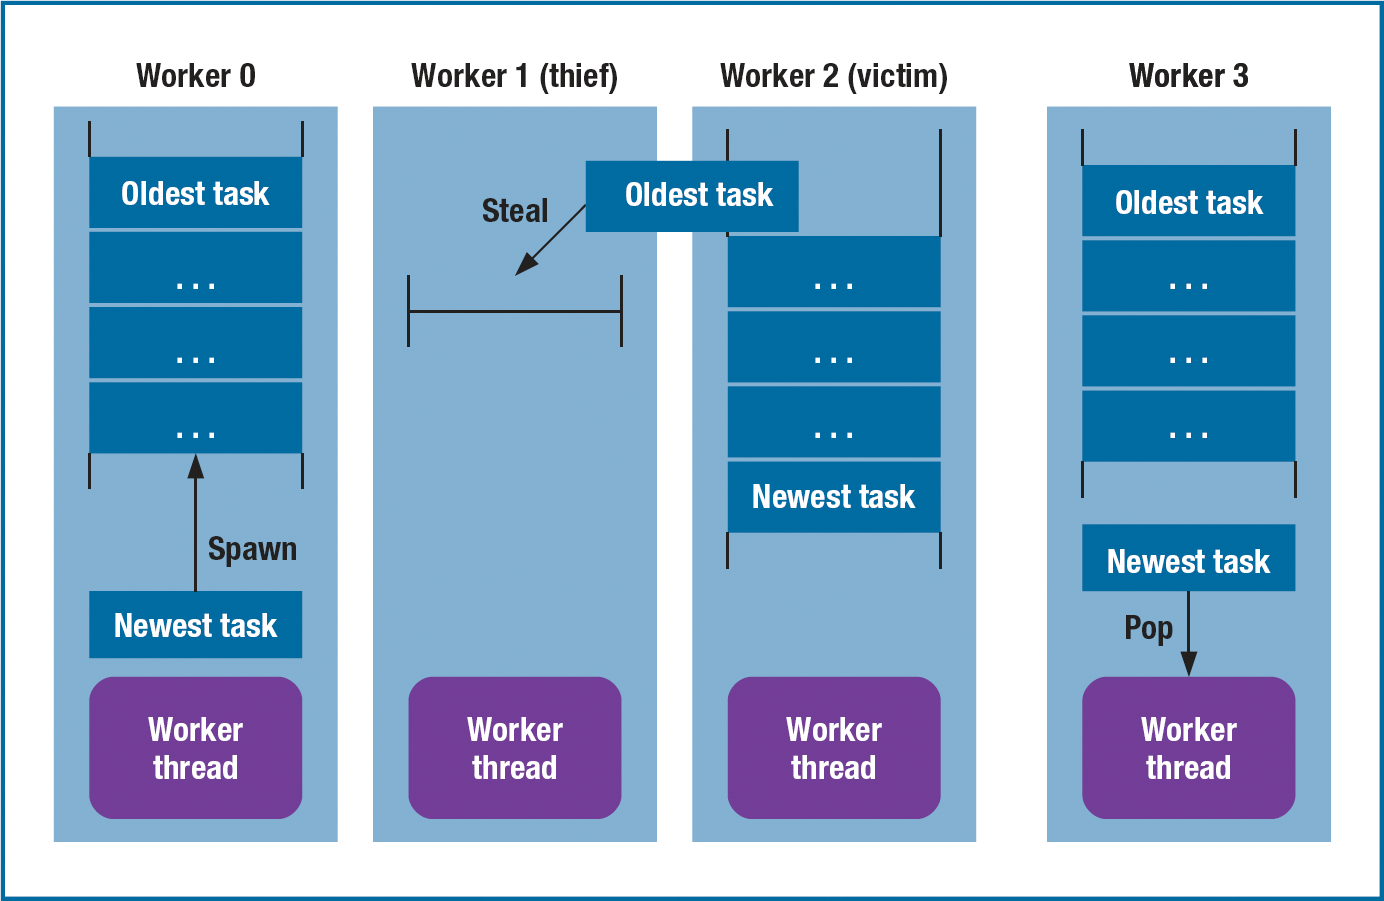
\includegraphics[width=0.7\linewidth]{fig/tbb.png}
\caption*{\small Fig source: \href{https://csdl-images.computer.org/mags/so/2011/01/figures/mso20110100232.gif}{Intel TBB}}
\end{figure}
\end{frame}

\subsection{SIMD}
\begin{frame}
\subsectionpage
\end{frame}

\begin{frame}{ILP}
\begin{itemize}
	\item Pipelining
	\item Hyperscalar
	\item Very Long Instruction Word (VLIW)
	\item Vector processing
	\item Out-of-Order (OoO) execution
	\item Spectacular execution
\end{itemize}
\end{frame}

\section{Distributed Parallelization}
\begin{frame}
\sectionpage
\end{frame}

\begin{frame}{MPI}

\end{frame}

\section{Parallel Computing Frameworks}
\begin{frame}
\sectionpage
\end{frame}

\begin{frame}{Frameworks}
\begin{itemize}
\item MapReduce
\item Spark
\item Ray
\end{itemize}
\end{frame}

\section{Summary}
\begin{frame}
\sectionpage
\end{frame}

\begin{frame}[fragile]{Summary}
\begin{itemize}
	\item Introduction
	\item Shared-memory: \verb'<pthreads>', OpenMP, Cilk, AVX
	\item Distributed-memory: MPI
	\item Parallel computing frameworks: MapReduce
\end{itemize}
\end{frame}

\end{document}